% Ledger-derived selection flow. Labels distinguish partial-text AI review.
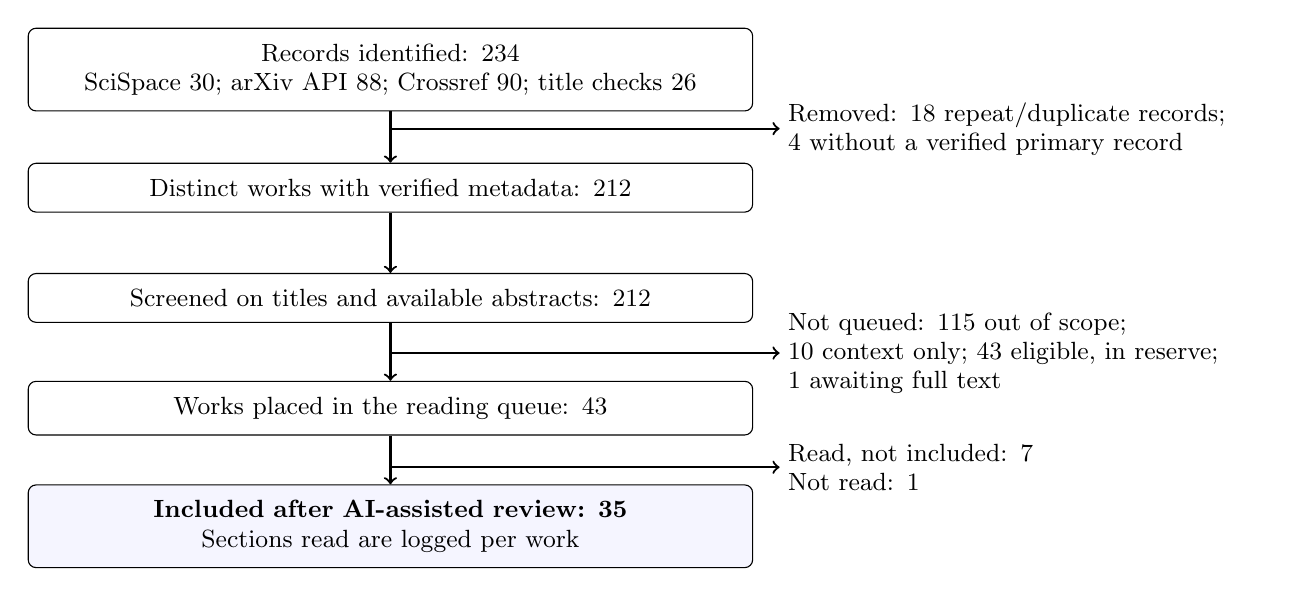
\begin{tikzpicture}[
 every node/.style={font=\fontsize{9}{10.5}\selectfont},
 box/.style={draw,rounded corners=1mm,align=center,text width=88mm,inner sep=2mm},
 note/.style={align=left,text width=59mm,inner sep=1mm},
 flow/.style={->,thick}]
\node[box] (a) at (0,0) {Records identified: 234\\SciSpace 30; arXiv API 88; Crossref 90; title checks 26};
\node[box] (b) at (0,-1.5) {Distinct works with verified metadata: 212};
\node[box] (c) at (0,-2.9) {Screened on titles and available abstracts: 212};
\node[box] (d) at (0,-4.3) {Works placed in the reading queue: 43};
\node[box,fill=blue!4] (e) at (0,-5.8) {\textbf{Included after AI-assisted review: 35}\\Sections read are logged per work};
\draw[flow] (a)--(b);\draw[flow] (b)--(c);\draw[flow] (c)--(d);\draw[flow] (d)--(e);
\node[note] (r) at (8.0,-.75) {Removed: 18 repeat/duplicate records;\\4 without a verified primary record};
\node[note] (q) at (8.0,-3.6) {Not queued: 115 out of scope;\\10 context only; 43 eligible, in reserve;\\1 awaiting full text};
\node[note] (n) at (8.0,-5.05) {Read, not included: 7\\Not read: 1};
\draw[flow] (0,-.75)--(r.west);\draw[flow] (0,-3.6)--(q.west);\draw[flow] (0,-5.05)--(n.west);
\end{tikzpicture}
